% Seeded from ../slides/lecture_33.tex; substantive frame content retained.
% Title and primary objective become handout metadata; presentation commands removed.
\documentclass[compact]{ne630handout}
\handoutsolutionsfalse
% Assigned reading: ../administrivia/schedule-source.psv.
\begin{document}
\Lesson{33}{One-Speed Diffusion in Heterogeneous Slabs}{FNRP 6.4.}{Students will be able to develop solutions for the one-speed diffusion equation in slab geometry for systems with multiple homogeneous regions subject to continuity conditions and boundary conditions (\emph{vacuum} and \emph{reflecting}).}
\begin{handoutflow}


% Source: lecture_33.tex, frame at line 90.
\Sec{1}{Review: Diffusion in a Homogeneous Slab}
Last time, we considered the one-speed diffusion equation
\begin{align*}
   \frac{d^2 \phi}{d x^2}
  - \frac{1}{L^2}\phi(x)
  = -\frac{S(x)}{D} \, \qquad \text{subject to} \qquad \phi(0) = \phi(a) = 0 \, ,
\end{align*}
where
\begin{equation*}
 L = \sqrt{\frac{D}{\Sigma_a}} \quad \text{and} \quad D = \frac{1}{3\Sigma_{tr}} \, .
\end{equation*}

For $S(x) = S_0$, we applied the ``algorithm''  to find the equivalent to
\begin{equation*}
 \phi(x)=\frac{S_0}{\Sigma_a}\left[1-\frac{\cosh\!\big(\tfrac{x-a/2}{L}\big)}{\cosh\!\big(\tfrac{a}{2L}\big)}\right] \, .
 \label{eq:ex1sol}
\end{equation*}

% Source: lecture_33.tex, frame at line 113.
\Sec{2}{Review: $\psi$, $\phi$, $\mathbf{J}$, and a new friend, $J^{\pm}$}
Skipping any proofs, diffusion theory in slab geometry leads to
\begin{align*}
  \psi(x, \theta)  &= \frac{1}{4\pi} {\phi}(x) + \frac{3}{4\pi} \overbrace{\cos(\theta) \, \hat{\mathbf{i}} \cdot \mathbf{J}(x)}^{J(x)} \\
\text{or} \quad \psi(x, \mu)   &= \frac{1}{4\pi} \phi(x) - \frac{3}{4\pi} \mu D \frac{d\phi}{dx}   \, ,
\end{align*}
where $x$ is the polar axis, $\theta$ is the polar angle, and $\mu = \cos(\theta)$.  It follows that
\begin{align*}
  \phi(x) &= \int^{2 \pi}_0 d\varphi \int^1_{-1} \psi(x, \mu) d\mu \quad \text{and} \quad
  J(x)    = \int^{2 \pi}_0 d\varphi \int^1_{-1} \mu \psi(x, \mu)  d\mu \, .
\end{align*}

Then the rightward (leftward) {\bf partial current} is defined as
\begin{align*}
 J^{\pm} = \int^{2 \pi}_0 d\varphi \int_{\mu \gtrless 0} \mu \psi(x, \mu)  d\mu \rightarrow
   \boxed{ J^{\pm} = \frac{1}{4}\,\phi(x) \mp \frac{D}{2}\,\frac{d\phi}{dx} }\, .
\end{align*}

{
{\bf Example}.  Write $\phi$ and $J$ in terms of $J^{\pm}$.  \\

{\bf Ans.} $\phi=(J^+ + J^-)/2$ and $J = J^+ - J^-$.
}

% Source: lecture_33.tex, frame at line 146.
\Sec{3}{Boundary Conditions:}
Three common scenarios at a boundary $x_b$
we want to model:

\begin{enumerate}
 \item {\bf vacuum} (empty space; no neutrons)
 \item {\bf reflection} (no net flow, i.e., $J(x_b) = 0$ or $(d\phi/dx)|_{x=x_b} = 0$)
 \item {\bf boundary source} (specified {\it inward} flow, i.e., $J^{in}(x_b) = S_b$)
\end{enumerate}

\par

\resizebox{\linewidth}{!}{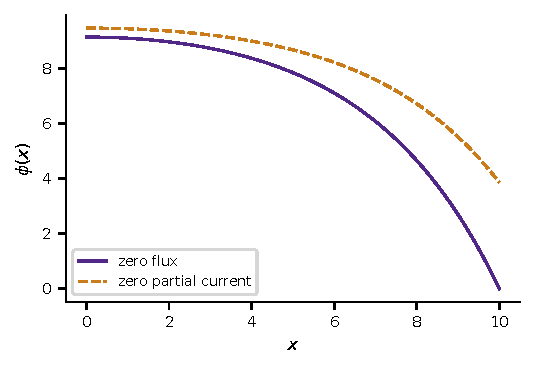
\includegraphics{figures/drafts/slab_bc.pdf}}

\par

\par

{ {\bf Example}: Solve $-D\phi'' + \Sigma_a \phi(x) + S_0$, subject to reflection at $x = 0$ and modeling vacuum at $x=a$ using (a) $\phi(a)=0$ and (b)  $J^{in}(b) = 0$. Plot both results for $a = 10$ cm, $S_0 = 1$ \si{\per\centi\meter\cubed\per\second}, $D = 1.0$ cm, and $\Sigma_a = 0.1$ \si{\per\centi\meter}.}
\par

Note that $J^{in}(a) = J^-(a) = 0$ is the natural way to define vacuum conditions!  On the other hand, the zero-flux condition $\phi(a)=0$ actually imposes a {\it negative} incident current that eats neutrons and decreases $\phi(x)$ everywhere! {\bf Avoid!}

% Source: lecture_33.tex, frame at line 178.
\Sec{4}{Continuity Conditions}
In addition to boundary conditions, we must maintain continuity of

\begin{enumerate}
 \item the scalar flux $\phi(x)$
 \item the current $J(x) = -D \frac{d\phi}{dx}$
\end{enumerate}

{\bf everywhere} in the domain--even across boundaries between
different material regions!

{\bf Example}. Consider a two-region slab with an interface at $x = a$.  For $x \lessgtr a$, denote the flux by $\phi^{\text{I}/\text{II}}$ and the diffusion coefficient by $D^{\text{I}/\text{II}}$.  Write down the two equations imposed by continuity.

{\bf Ans}. Flux continuity requires $\phi^{\text{I}}(a) = \phi^{\text{II}}(a)$, while current continuity requires
$-D^{\text{I}} \frac{d\phi^{\text{I}}}{dx}\Big |_{x=a} = -D^{\text{II}} \frac{d\phi^{\text{II}}}{dx}\Big |_{x=a}$.
Importantly, this means that the flux gradient {\it can} exhibit discontinuities (if $D^{\text{I}} \neq D^{\text{II}}$)!

\end{handoutflow}
\end{document}
